\documentclass[12pt,letterpaper]{article}
\usepackage[utf8]{inputenc}
\usepackage{amsmath}
\usepackage{amsfonts}
\usepackage{amssymb}
\usepackage{graphicx}
\usepackage{fancyhdr}

\lhead{\begin{picture}(0,0) \put(0,0){
\includegraphics[width=20mm]{./n1.png}} \end{picture}}
\renewcommand{\headrulewidth}{0.5pt}

%\chead{Nuevas Ideas Tecnológicas}

\pagestyle{fancy}

\renewcommand{\familydefault}{\sfdefault}
\title{Propuesta Técnica}
\author{N.I.T.\\
Camarillo Martínez Jazmin\\
García Martínez Isaac\\
Hernández Valerdi Daniel\\
Gutiérrez Bárcenas Francisco\\
Quiroz Luis}
\begin{document}
\maketitle

\newpage 
\tableofcontents
\newpage 
\section{CONTEXTO:}
"Consorcio Deportivo S.A. de C.V."  es una empresa nueva, que busca crecer a nivel nacional, para esto se unió con otras cadenas deportivas. Al poner en funcionamiento sus gimnasios en Monterrey, Guadalajara y en la Ciudad de México, se dieron cuenta que las demás cadenas tienen procesos, procedimientos e información diferentes; algunas personas que viajan y que quieren seguir con su rutina de ejercicio, se les negó el ingreso a las instalaciones ya que la información no se encuentra unificada en todas las sucursales.

Las actividades que pueden ser "contratadas" tienen problemas ya que no tienen control alguno. Estas actividades son: área de piscina, área de instrumentos (pesas, caminadoras, etc.), área de canchas (fútbol, tennis, etc.).  De igual manera las membresías carecen de control alguno, ya que los miembros no ponen atención a la fecha de renovación de estas. Los miembros a los que se les notificó que tenían su pago de renovación atrasado se les negaba su ingreso a lo que el miembro se respalda tras la escusa que ya realizó el pago, ya que no hay manera de comprobar de manera inmediata la veracidad de esto, se le da acceso al cliente, esto se traduce en pérdidas.


\section{DESCRIPCIÓN DE LOS PROBLEMAS:}
A continuación se mencionaran detalladamente cada uno de los problemas vistos, así como diagramas de problemas con sus respectivas consecuencias.
\begin{itemize}
    \item Unificación de la información y estandarización de procesos:
Debido a la incorporación de diferentes sucursales existentes, no hay información accesible ni una regularización en la actualización de los datos, lo cual impide la unificación de todas las entidades, causando así ambigüedad en datos y confusión para los empleados llevando a esto la ineficiencia del trabajo.
    \item Gestión de clientes: 
Consiste en la unión de más sucursales deportivas ya que se van adquiriendo nuevas necesidades en cuanto a la adquisición de membresías, ya que cuando se genera un pago de esta no se ve reflejado al instante para poder saber si el cliente tiene acceso al deportivo, generando así pérdida de tiempo en lo que se solicita información al personal adecuado, provocando molestia en los clientes e incluso la baja de dicho cliente.
\item Gestión de actividades: 
    \begin{itemize}
    \item Debido al acceso al deportivo en diferentes horarios, no se tiene un límite de cupo en las múltiples áreas del deportivo, ni tampoco un límite al usar las instalaciones, provocando así la saturación de las áreas como lo son; salones, canchas, piscina, etc.
    \item Para cada tipo de sucursal hay diferentes tipos de ubicación y espacio donde se imparten las actividades, por lo cual no hay forma de saber en dónde se impartirá un cierto tipo de curso o clase. A demás de que no todas las actividades aceptan edades mixtas, causando una mala distribución de clientes para las diferentes actividades, o el cierre de esta.
    \end{itemize}
\end{itemize}
A continuación se presentará un diagrama donde se podrán ver de manera esquemática los diferentes tipos de problemas.\\ \\ \\ \\ \\ \\ \\ \\ \\ \\ \\ \\ \\ \\ \\ \\ \\ \\ \\ \\ \\ \\ \\

\begin{figure}
   \centering
   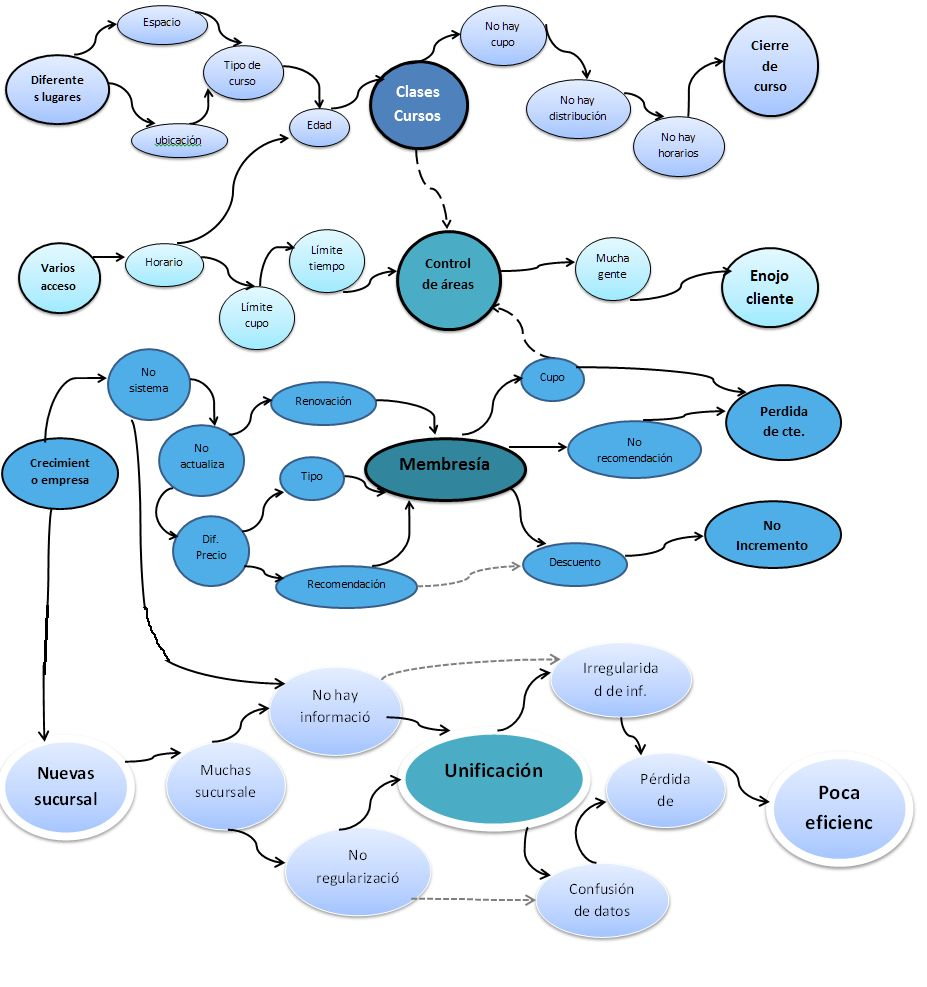
\includegraphics[scale=0.50]{problemas.png}
   \caption{Problemas encontrados}
   \label{fig:my_label}
\end{figure}


\section{OBJETIVOS}
Una vez establecido los problemas, nos queda a nosotros ponernos como objetivo resolver dichos problemas.
\subsection{Objetivo general.}
Brindar al Consorcio Deportivo S.A. de C.V. una herramienta la cual pueda facilitar el manejo de información de sus clientes y áreas en las diferentes sucursales que tiene alrededor del país.
\subsection{Objetivos Específicos.}
	\begin{itemize}
	
	\item Implementar una base de datos para administrar la información de los clientes, áreas,sucursales y personal.
	
	\item Desarrollar un sistema web con una interfaz gráfica para que los trabajadores puedan acceder a la información necesaria para las diferentes áreas y actividades que se realizan en las diferentes sucursales.

	\item Organizar en la Base de datos los horarios de las actividades(curso/clases) en las diferentes sucursales.
	
	\item Verificar por medio del sistema web que los pagos se hayan efectuado correctamente.	
	
	\item Establecer un mecanismo para validar el derecho de ingreso a las sucursales.
	
	\end{itemize}


\subsection*{Propuesta para  la  unificación de procesos y procedimientos.} 
La siguiente parte del documento tiene la finalidad de mostrar una propuesta para un sistema de unificación  el cual está compuesto por estos principales aspectos.

\begin{itemize}
    \item Desarrollo de aplicación web.
    \item Base de datos centralizada.
    \item Cloud hosting.
    \item Manuales de proceso y de usuario
\end{itemize}


El sistema integración está pensado para una plataforma web la cual tiene el siguiente cuadro comparativo de ventajas y desventajas que nos guiaron para tomar la decisión fundamental para la propuesta:

\subsection*{Ventajas}

    \begin{itemize}
        \item Disponibilidad de la información en cualquier parte en la que se tenga Internet.
        \item No requiere ser instalado.
        \item Mantenimiento y soporte a distancia sin premuras de transporte, climatológicas, etc.
        \item Disponible para cualquier sistema operativo (PC, Mac, Linux), celular (Android, iPhone, etc.) y cualquier otro dispositivo que tenga acceso a Internet.
        \item Multiusuario, pueden estar conectados un número ilimitado de usuarios al sistema y guardar la configuración, acceso y registro de las acciones que se llevan a cabo en el sistema.
        \item Se evita la compra de un servidor dedicado y el costo de luz y mantenimiento del mismo.
        \item Se evita la compra de un servidor dedicado y el costo de luz y mantenimiento del mismo.
        \item Sustituye procedimientos manuales que consumen tiempo y energía del equipo de trabajo.
        \item Escalabilidad en CPU, RAM y almacenamiento para el servidor.
    \end{itemize}


\subsection*{Desventajas}
    \begin{itemize}
        \item Requiere acceso a internet para consultar la información y hacer uso de sistema.
        \item No disponibilidad del sitio por problemas con el proveedor de hosting.
        \item Los tiempos de repuesta están determinados por el proveedor de Internet.
    \end{itemize}



\section{Propuestas para los cursos:}
	Proponemos usar restricciones para cada tipo de curso, las restricciones que vamos a tomar en cuenta son las siguientes:	
		\begin{itemize}
			\item Edad: porque ciertas actividades que tendrán los gimnasios no son aptos para todo el público.
			\item Tipo del curso: así podrán saber que cursos se darán en las sucursales.
			\item Hora: con esto se puede tener el control sobre los cursos para que con el sistema web los clientes puedan revisar qué hora les acomoda y los empleados puedan resolver un inconveniente con un cliente que haya faltado a una clase.
			\item Espacio: registraremos las medidas de los espacios destinados para los cursos y las clases.
			\item Cupo: Con el cupo podrán resolver si pueden ofrecerle a un cliente una reposición de una clase o si puede entrar a un curso.
			\item Ubicación de la sucursal: Utilizaremos la ubicación de las en el sistema para comparar los servicios que estas dan y que se pueda orientar a un cliente si se va a otra sucursal. 
			\item Lugar del espacio utilizado para las clases o cursos: Se tendrá el control de los espacios para saber si se puede ocupar por cualquier persona el tiempo que desee o se tendrá una limitante.
		\end{itemize}
			
			Dependiendo de la sucursal en la que se imparte el curso son las restricciones que se revisara el sistema con los datos obtenidos desde la base de datos, con lo cual esas características y restricciones las vamos a incluir en el modelo de la base de datos y así se simplificara el control sobre cuantas personas pueden estar en las clases y cursos y que requisitos necesitan para poder ingresar.
\section{Propuesta para las membrecías}
    Se proponen tres tipos de solución de acuerdo con las reglas del negocio y las especificaciones que se identificaron las cuales son:
    \subsection*{Renovaciones:}
        \begin{itemize}
            \item Se establecerán alertas mediante correo electrónico a cada usuario que no hayan efectuado su pago mensual una semana antes de que se les niegue la entrada en el establecimiento, esta alerta será enviada a su correo electrónico registrado al momento de su inscripción.
            \item Se generará un archivo de texto plano con los clientes que están por vencer sus membresías, esto con el fin de analizar y tomar acciones para la permanencia de los clientes.
            \item Se podrá renovar solo de 3 maneras, de forma mensual, anual y semestral, también se podrán adelantar renovaciones por un 
        \end{itemize}
    \subsection*{Tipo:}
        \begin{itemize}
            \item Se establecerán 5 tipos de membrecía, las cuales serán diferentes en precio y privilegios dentro de las instalaciones, el cliente no podrá modificar o agregar privilegios a las membresías, solo podrá cambiar su tipo de membrecía siempre y cuando sus pagos se encuentren al corriente.
        \end{itemize}
    \subsection*{Recomendaciones:}
        Cualquier cliente podrá recomendar los servicios del establecimiento invitando a un conocido o familiar, se le otorgará un descuento en su membrecía siempre y cuando el invitado haga uso de alguno de nuestros servicios o se compre algún tipo de membrecía, los descuentos pueden ser acumulables siempre y cuando el cliente no cuente con adeudos

			
\section{Plan de alcance}
\subsection{Requerimientos funcionales y no funcionales:}

\begin{itemize}
	\item RF1 Clientes
	\\ El sistema deberá almacenar en la base de datos a través de formularios los siguientes datos de los clientes: Nombre, Domicilio, correo, curp, teléfono, numero de emergencia, fecha de nacimiento y algunos datos médicos como: estatura, peso, alergias y enfermedades crónicas, si toma algún medicamento. Ya que con estos datos podrán tener una mejor comunicación con el cliente y reaccionar ante alguna emergencia de forma oportuna.
	\\ Prioridad: Alta.
	
	\item RF2 Áreas
	\\ El sistema deberá almacenar en la base de datos información de áreas como: capacidad máxima de personas, encargado de área, actividades impartidas, la sucursal donde se encuentra, horarios. Con estos datos se podrá organizar las actividades que se realizarán.
	\\Prioridad: Alta.
	
	\item RF3 Sucursal
	\\ El sistema deberá almacenaren la base de datos información correspondiente a las sucursales como son: la ubicación, servicios con los que cuenta, catálogo de clientes , horarios de servicio, contacto. Pensado en la movilidad de clientes y personal entre las diferentes sucursales.
	\\Prioridad: Media.
	
	\item RF4 Personal
	\\ El sistema deberá contar con tipos de roles como lo son: administradores y usuario estándar. Los administradores tendrán las facultades de modificar, eliminar y agregar datos a la base de datos. Mientras que el usuario estándar solo podrá visual los datos.
	\\Prioridad: Media. 
	
	\item RF5 Interfaces gráficas
	\\El sistema desplegara las pantallas con la información que se almacenará en la base de datos correspondiente a los clientes, áreas y sucursales. La interfaz gráfica deberá tener un botón de modificar, solo para aquellos usuarios que tengan permiso para realizar esa operación. Para que el personal que dese ver esta información pueda verla o modificar la información almacenada.
	\\Prioridad: Media
	
	\item RF6 Actividades
	\\El sistema deberá tener almacenado en una tabla el horario de cada actividad que se realice en las sucursales que hay, teniendo los siguientes datos: Sucursal, Nombre de actividad, quien imparte la actividad, día y hora en la que es impartida. Para que cada inicio de curso se pueda llenar la tabla con la información correspondiente y los encargados de cada actividad tengan conocimiento de sus horarios. 
	\\Prioridad: Media
	
	\item RF7 Aviso de Pago de Membresía
	\\El sistema debe tener un modulo de pago el cual consistirá informar al cliente una semana antes de que termine su membresía por medio de un correo electrónico. Para que el cliente pueda estar informado que su membresía esta por vencer.
	\\Prioridad: Media
	
	\item RF8  Pago de Membresía
	\\El sistema deberá desplegar una pantalla que muestre los campos de Nombre del cliente, apellidos y el número de membresía, para checar que el pago se haya realizado o para efectuar pagos ahí.  
	\\Prioridad: Alta
	
	\item RF9 Ingreso
	\\El sistema debe encargarse de tener la conexión entre el código QR y el lector, para poder permitir el acceso al cliente que haya efectuado su pago a tiempo.
	\\Prioridad: Alta
	  
	
	\item RNF 1: El usuario de las instalaciones del gimnasio deberá llevar su identificación en todo momento para conocer toda la información referente al usuario.
\item RNF 2: Un usuario puede entrar a todas las sucursales pertenecientes a la cadena. 
\item RNF 3: El cliente necesariamente debe de propocionar toda la información que el negocio requiera.
\item RNF 4: Cada actividad debe de tener un encargado.
\item RNF 5: Las áreas de canchas, piscina, salón de usos múltiples, debe tener un limite de 15 personas.
\item RNF 6: Para el acceso a cada área es necesario el código QR que viene en la membresía.
\item RNF 7: En caso de no haber comprobación alguna del pago correspondiente a la membresía, se le negará el acceso a las instalaciones.
\item RNF 8: El usuario debe ser el encargado de poder actualizar su información.
\item RNF 9: Para poder generar el ID de cada usuario, se tomarán las letras iniciales de sus apellidos y de sus nombres, así como la fecha de nacimiento.
\item RNF 10: Cada membresía debe ser limitado por color dependiendo del tipo. 	
\item RNF 11: El sistema deberá iniciarse correctamente con los navegadores web siguientes: Chrome, Firefox, Safari, Opera en las versiones (actuales).
\item RNF 12: El sistema deberá poderse ejecutar en diferentes entornos, como Windows, Linux, etc. (Multiplataforma).	 
\item RNF 13: El sistema necesitara al menos de una computadora de escritorio con memoria de 4Gb en RAM y un procesador Celeron de quinta generación o superior.
\item RNF 14: El sistema deberá de comunicarse con las otras sucursales a través de Internet sin importar la computadora.
	 
\end{itemize}

\section{Plan de tiempo}
A continuación se mostrará como es que vamos a realizar el sistema en cuestión de tiempo a través del siguiente diagrama de gantt.
\\ \\ \\ \\ \\ \\ \\ \\

\section{Plan de Capital Humano}
Para realizar el sistema es necesario contar con el personal adecuado para realizar dicho sistema, es lo que se presentará a continuación, reafirmando lo mostrado en la figura dos con nuestro organigrama.\\

	\begin{itemize}
	\item Gerente de proyecto. 
	\item Líder de proyecto.
	\item Programador.
	\item Diseñador Front-End.
	\item Analista y administrador de base de datos.
	\end{itemize}
	 
	
\begin{figure}
   \centering
   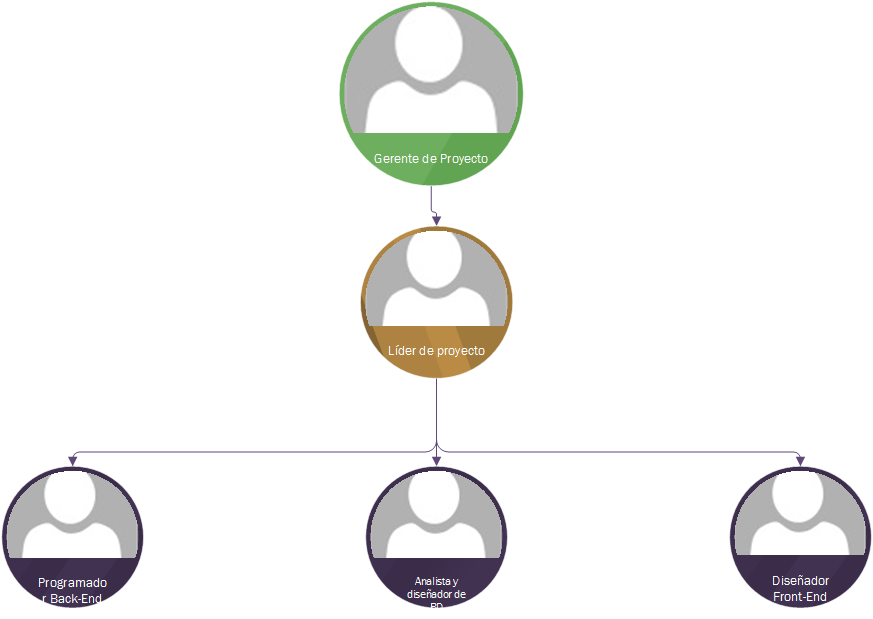
\includegraphics[scale=0.50]{Organigrama.png}
   \caption{Organigrama}
   \label{fig:my_label}
\end{figure}
\subsection*{Gerente de proyecto}
Puesto: Gerente de Proyecto\\ 
Edad: 30-45\\
Sexo: indistinto\\
Escolaridad: Carrera Profesional (título) relacionada con Tecnología de la Información, maestría en administración deseable.\\
Conocimientos: \\
Conocimiento y aplicación de metodologías PMP y agiles en la gestión de proyectos de desarrollo SW. 
Conocimiento y experiencia en metodología SCRUM. 
Conocimiento de modelado en bpm
Liderar el equipo interno de gestión de proyectos estratégicos 
Trabajar en equipo para guiar a los compañeros de trabajo que brindan su aporte a los planes de desarrollo.\\
Experiencia:  5 años en puesto similar. \\
Sueldo: 30000 a 40000\\
\subsection*{Líder de proyecto}
Edad: 30-40 años\\
Escolaridad: ingeniera en ISC, Informática o a fines.\\
Sexo: Indistinto\\
Requisitos:\\
Experiencia de al menos 3 años desarrollando sistemas en la plataforma J2EE aplicando de forma correcta los conceptos de orientación a objetos.\\
Conocimientos  basadas en las siguientes tecnologías de J2EE: servlets, JSP, JSF, JMS, EJB o métodos de persistencia.
Experiencia  con frameworks de desarrollo Web como Struts, Spring o WebWorks o similar.
Experiencia en desarrollo de soluciones a través de la implementación de Web Services
Conocimientos en la documentación del código fuente de las aplicaciones desarrolladas (no generadores automáticos) así como el manejo de sistemas de control de versiones como 
CVS o Subversión.
Conocimiento  utilizando Servidores de aplicaciones como Tomcat, Websphere o Weblogic.
Conocimiento de lenguaje UML.\\
Sueldo: 25,000.00\\

\subsection*{Programador}
Puesto: Programador back end\\
Edad: 20-35 años\\
Escolaridad: Ingeniera en ISC o a fines, recién egresados o titulados\\
Experiencia: mínimo 1 año\\
Requisitos:\\
Conocimiento de lenguajes de programación orientado a objetos y framework de desarrollo web 
Principales actividades
Desarrollo de aplicaciones Web\\
Tipo de contrato: por un año\\
Sueldo: 16,000\\
Vacantes 2

\subsection*{Diseñador Front-End}
Edad: 25- 30 años\\
Escolaridad: Diseño Gráfico, Comunicación Gráfica, Diseño y Comunicación Visual; titulado.\\
Sexo: Indistinto\\
Requisitos:\\
Se necesita Director creativo que sepa manejar herramientas de desarrollo como html5, boostrapt, jquery, css y creación y edición de imágenes con Photoshop, Ilustrator. Tenga 
como experiencia mínima de 3 años, sepa hablar inglés básico.\\ 
Sueldo: 10,000.00 

\subsection*{Analista y administrador de base de datos}
Puesto: analista y administrador de base de datos\\
Edad: 25 a 35\\
Sexo: indistinto\\
Escolaridad:: Ing. en Sistemas Computacionales o licenciatura en informática o a fin.
Requisitos: Atención de requerimientos para funcionalidad
Manejo de base de datos Optimización de procesos de BD Análisis de información,
Migración de códigos Creación y modificación de tablas, vistas, funciones, triggers, store procedure, Jobs
Elaboración y mantenimiento a procedimientos almacenados en bases de datos.
Tecnologías: Oracle, SyBase, SQL Server, MySQL
Experiencia:  2 años 
Sueldo: 15000 a 20000

\section{Plan de costo}
En eta sección manejaremos un estimación de costos de los recursos materiales y humanos que se utilizaran para el desarrollo del sistema. Las siguientes tablas mostraran la información obtenida.\\\\  \\\\\\\\ \\\\\\\\\\\\\\\\\\\\\\\\\\\\\\\\\\\
\begin{figure}
   \centering
   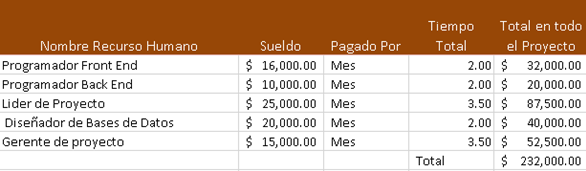
\includegraphics[scale=1.00]{tabla1.png}
   \caption{Recursos Humanos}
   \label{fig:my_label}
\end{figure}

\begin{figure}
   \centering
   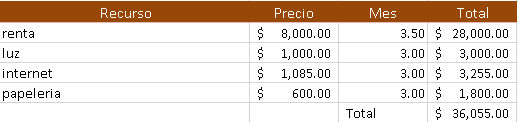
\includegraphics[scale=1.00]{tabla2.png}
   \caption{Insumos}
   \label{fig:my_label}
\end{figure}

\begin{figure}
   \centering
   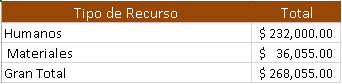
\includegraphics[scale=1.00]{tabla3.png}
   \caption{Total de costos}
   \label{fig:my_label}
\end{figure}

\end{document} 